%----------------------------------------------------------------------------------------
%	PACKAGES AND THEMES
%----------------------------------------------------------------------------------------
\documentclass[aspectratio=169,xcolor=dvipsnames]{beamer}
\newcommand{\singlelinelogo}{\setbeamertemplate{logo}{
    \begin{picture}(0,0)
            \put(0,0){\makebox(-60,235)[rt]{
\includegraphics[width=2.8cm]{images/logos/unibg-logo.png}}}
             \put(0,0){\makebox(-20,236)[rt]{
\includegraphics[width=0.9cm]{images/logos/gaps.png}}}
        \end{picture}
}}

\newcommand{\sectiontitlelogo}{\setbeamertemplate{logo}{
    \begin{picture}(0,0)
            \put(0,0){\makebox(-205,220)[rt]{
\includegraphics[width=2.8cm]{images/logos/unibg-logo.png}}}
             \put(0,0){\makebox(-165,221)[rt]{
\includegraphics[width=0.9cm]{images/logos/gaps.png}}}
    \end{picture}
}}

\newcommand{\backupbegin}{
   \newcounter{finalframe}
   \setcounter{finalframe}{\value{framenumber}}
}
\newcommand{\backupend}{
   \setcounter{framenumber}{\value{finalframe}}
}

\newcommand\T{\rule{0pt}{2.6ex}}       % Top strut
\newcommand\B{\rule[-1.2ex]{0pt}{0pt}} % Bottom strut

\usetheme{SimplePlus}

\usepackage{xcolor}
\usepackage{hyperref}
\usepackage{graphicx} % Allows including images/logos
\usepackage{booktabs} % Allows the use of \toprule, \midrule and \bottomrule in tables
\usepackage{comment}
\usepackage{tikz}
\usepackage{mhchem}
\usepackage{setspace}
\usepackage{array}
\newcolumntype{L}[1]{>{\raggedright\let\newline\\\arraybackslash\hspace{0pt}}m{#1}}
\newcolumntype{C}[1]{>{\centering\let\newline\\\arraybackslash\hspace{0pt}}m{#1}}
\newcolumntype{R}[1]{>{\raggedleft\let\newline\\\arraybackslash\hspace{0pt}}m{#1}}

\usepackage{setspace}
\usepackage{siunitx}
\sisetup{detect-all}

\newcommand{\greencheck}{{\color{ForestGreen}\checkmark}}


%----------------------------------------------------------------------------------------
%	TITLE PAGE
%----------------------------------------------------------------------------------------

\title[]{\large{Characterisation of the readout electronics of the Si(Li) tracker\\ for the first flight of the GAPS experiment}} % The short title appears at the bottom of every slide, the full title is only on the title page

\author[Luca Ghislotti] {Luca Ghislotti\\Master Thesis Defence\\ \vspace{0.3cm}\small September $30^{\text{th}}$, 2022}

\institute[UniBG]{
    \\Supervisor: prof. Massimo Manghisoni \\
    Co-Supervisors: Ph.D. Elisa Riceputi, Ms.C. Paolo Lazzaroni
}

\date{Computer Engineering\\Academic Year 2021/2022} % Date

% title page logos
\titlegraphic { 
    \begin{picture}(0,0)
        % VERSION WITH UNIBG AND GAPS LOGOS
        %\put(25,165){\makebox(0,0)[rt]{
\includegraphics[width=4cm]{images/logos/unibg-logo.png}}}
        %\put(90,168){\makebox(0,0)[rt]{
\includegraphics[width=1.4cm]{images/logos/gaps.png}}}
    
        % VERSION WITH ALL LOGOS
        \put(-110,165){\makebox(0,0)[rt]{
\includegraphics[width=3.6cm]{images/logos/unibg-logo.png}}}
        \put(-54,168){\makebox(0,0)[rt]{
\includegraphics[width=1.3cm]{images/logos/gaps.png}}}
        \put(16,168){\makebox(0,0)[rt]{
\includegraphics[width=2cm]{images/logos/nasa-logo.png}}}
        \put(79,163){\makebox(0,0)[rt]{
\includegraphics[width=2cm]{images/logos/jaxa-logo.png}}}
        \put(143,161){\makebox(0,0)[rt]{
\includegraphics[width=1.8cm]{images/logos/infn-logo.png}}}
        \put(210,161){\makebox(0,0)[rt]{
\includegraphics[width=1.8cm]{images/logos/asi-logo.jpg}}}
    \end{picture}
}

% all pages logos
\logo{
    \begin{picture}(0,0)
        \put(0,0){\makebox(-60,230)[rt]{
\includegraphics[width=2.8cm]{images/logos/unibg-logo.png}}}
         \put(0,0){\makebox(-20,231)[rt]{
\includegraphics[width=0.9cm]{images/logos/gaps.png}}}
    \end{picture}
}

%----------------------------------------------------------------------------------------
%	SLIDE: TITOLO, SOMMARIO e CONTENUTI
%----------------------------------------------------------------------------------------

\begin{document}

% TITOLO
\frame[plain]{
    \vspace{-0.5cm}
    \titlepage
}

% SOMMARIO
{\singlelinelogo
\begin{frame}{Overview}
    % Throughout your presentation, if you choose to use \section{} and \subsection{} commands, these will automatically be printed on this slide as an overview of your presentation
    %\setstretch{2.0}
    \tableofcontents
\end{frame}
}

%----------------------------------------------------------------------------------------
%	The GAPS Experiment
%----------------------------------------------------------------------------------------

\section{Introduction}
\subsection{The GAPS experiment}

{\singlelinelogo
\begin{frame}{The GAPS experiment}
\vskip0.2cm
\fontsize{9pt}{1}\selectfont
   \begin{columns}
   \vspace{0.05cm}
    \column{0.55\textwidth}
        \textbf{Scientific background}
        \vspace{0.05cm}
        \begin{itemize}
            \item One of the great unanswered questions in physics and astronomy concerns the properties and composition of dark matter
            \item Unlike normal matter, dark matter does not interact with the electromagnetic force. This means it does not absorb, reflect or emit light, making it extremely hard to spot
            \item A very promising indirect signature of dark matter are cosmic ray antideuterons
        \end{itemize}
        
        \vspace{0.2cm}
        \textbf{The experiment}
        \vspace{0.05cm}
        \begin{itemize}
            \item The General Antiparticle Spectrometer (GAPS) is an Antarctic balloon experiment designed to detect low-energy cosmic antinuclei as an indirect signature of Dark Matter
            \item Prototype flight (pGAPS) in 2012 at the JAXA balloon facility in Taiki, Japan
            \item First balloon flight from McMurdo Station in Antarctica in late 2023 (launch approved by NASA)
        \end{itemize}
        
    \column{0.4\textwidth}
        \begin{figure}
        \centering
        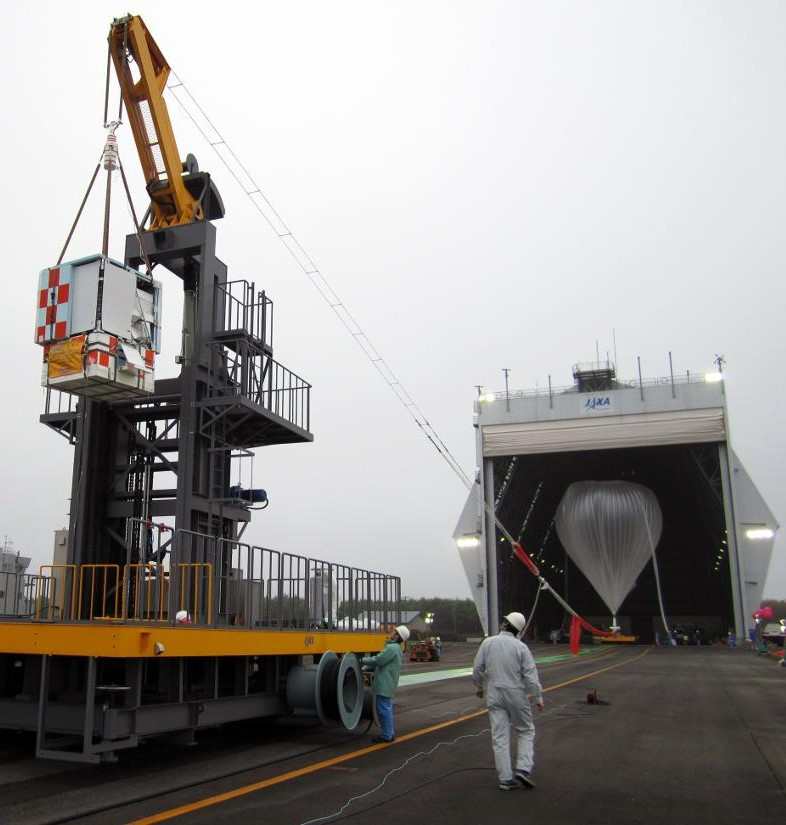
\includegraphics[height=0.64\textheight]{images/experiment_intro/gaps_balloon.jpg}
        \end{figure}
    \end{columns}
\end{frame}
}

\subsection{The GAPS instrument}

{\singlelinelogo
\begin{frame}{The GAPS instrument}
\fontsize{9pt}{1}\selectfont
   \begin{columns}
    \column{0.65\textwidth}
        \textbf{Time-of-Flight System (TOF)} 
        \begin{itemize}
            \item Composed of 220 plastic scintillator paddles
        \end{itemize}
        \textbf{Si(Li) Tracker}
        \begin{itemize}
            \item About 1440 Lithium-drifted Silicon, Si(Li), detectors
            \item 10 layers with \SI{10}{\cm} spacing
            \item 12x12 Si(Li) detectors per layer
            \item Modular structure (360 modules)
        \end{itemize}    
        \vspace{0.2cm}
        \textbf{Particle identification} \\
        \vspace{0.15cm}
        Time-of-flight system measures velocity and dE/dx \\
        \vspace{0.2cm}
        Si(Li) Tracker functions as:
        \begin{itemize}
            \item \textbf{target} to slow an incoming antiparticle and capture it into an exotic atom in an excited state
            \item \textbf{spectrometer} for de-excitation X-rays
            \item \textbf{tracker} to measure antinucleus dE/dx and stopping depth, and annihilation products from nuclear decay
        \end{itemize}
           
    \column{0.3\textwidth}
    \begin{picture}(0,0)
        \put(120,95){\makebox(0, 0)[rt]{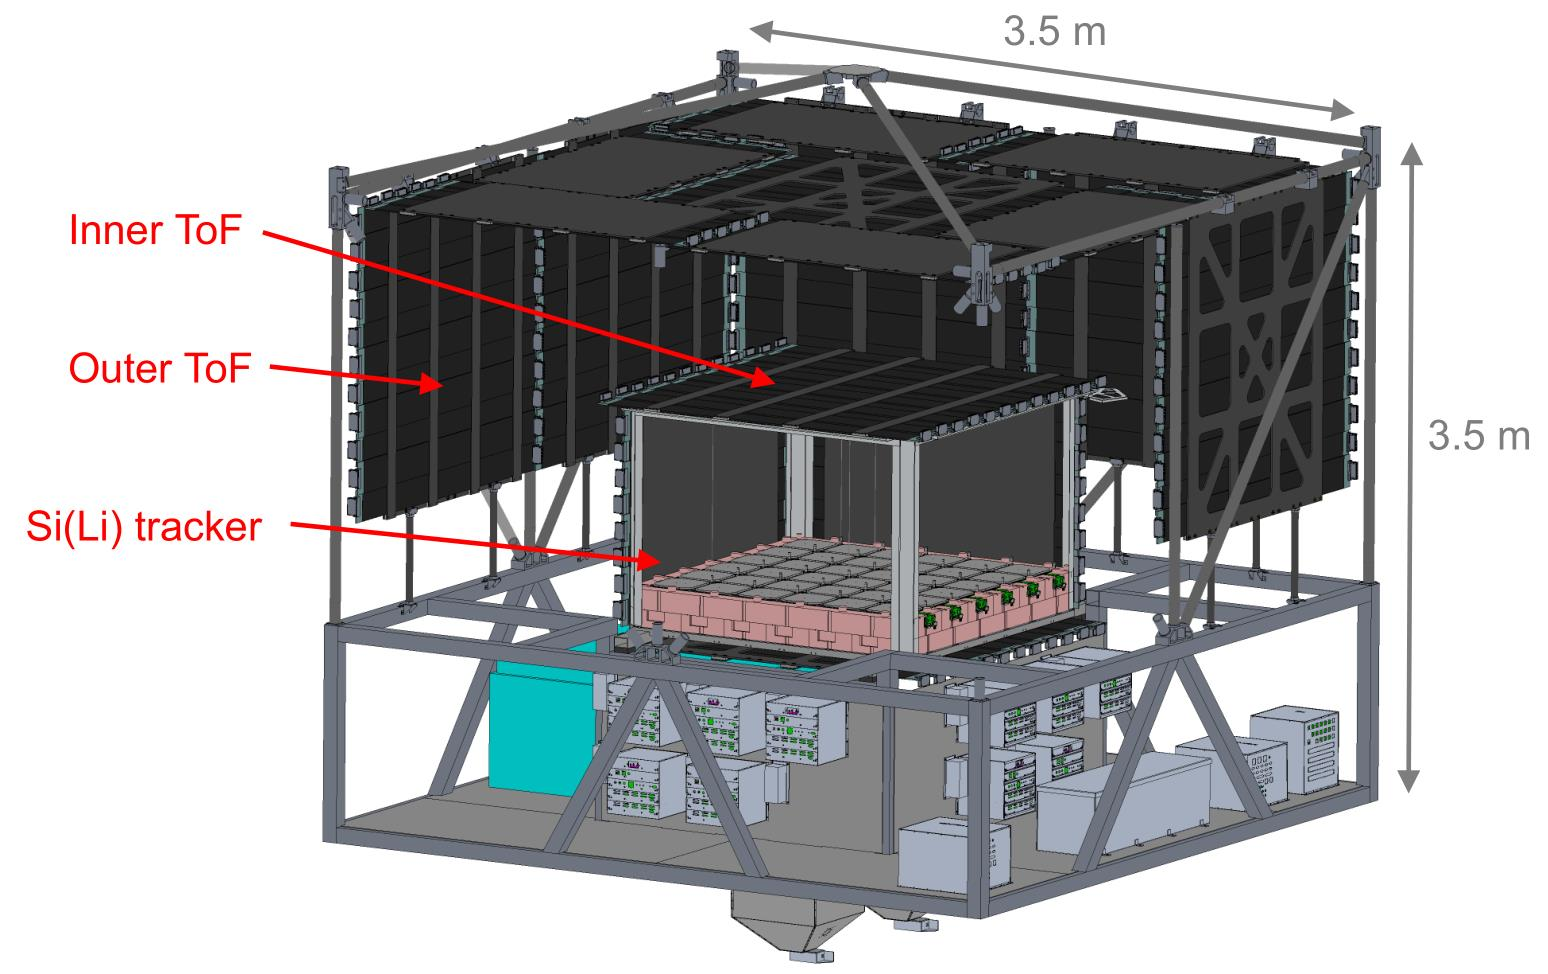
\includegraphics[width=5.8cm]{images/experiment_intro/GAPS_tracker_structure.jpg}}}
        \put(115,-23){\makebox(0, 0)[rt]{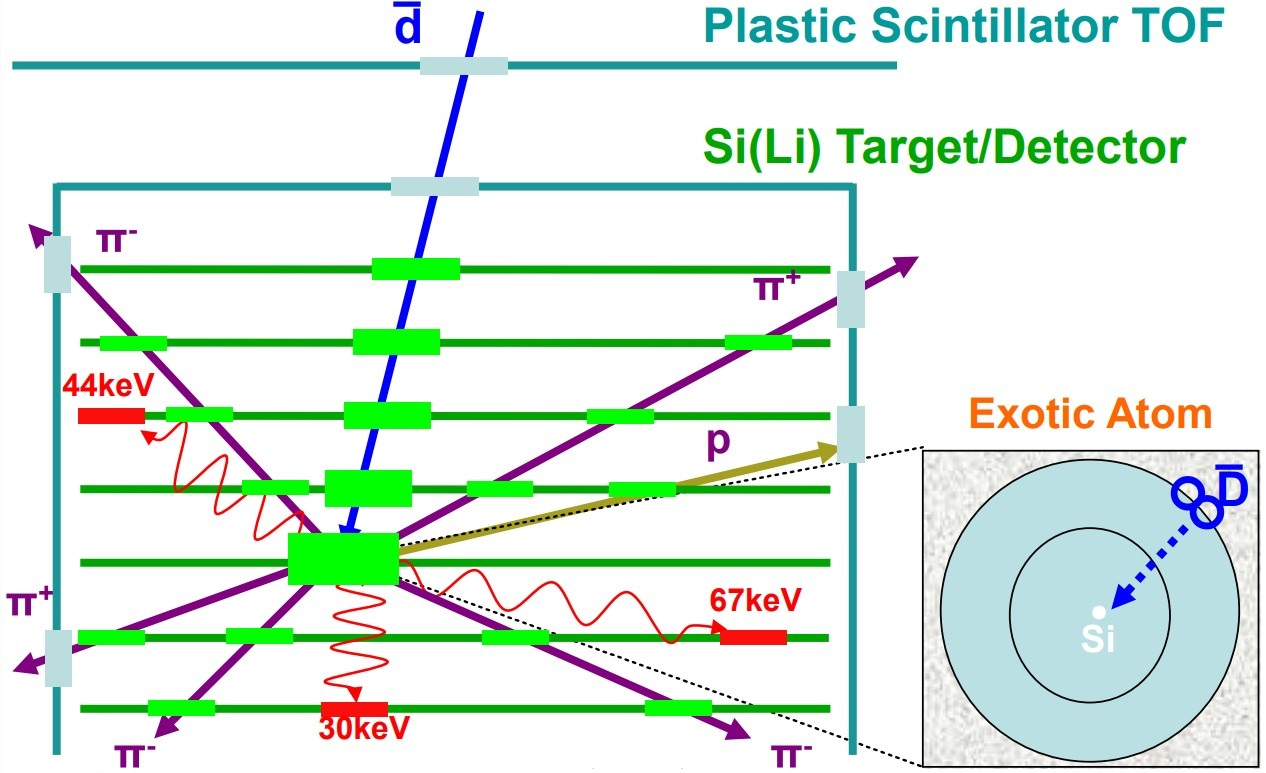
\includegraphics[width=4cm]{images/experiment_intro/GAPS_tracking_scheme.jpg}}}
    \end{picture}
    \end{columns}    
\end{frame}
}

\subsection{Si(Li) tracker module}

{\singlelinelogo
\begin{frame}{Si(Li) tracker module}
\fontsize{9pt}{1}\selectfont
   \begin{columns}
    \column{0.6\textwidth}
        \vskip0.2cm
        \textbf{Si(Li) tracker module structure} \\
        \vspace{0.15cm}
        Each module is composed by 4 Si(Li) detectors divided in 8 strips, the ASIC for the readout electronics and the Front-End Board (FEB) that allows the communication between the ASIC and the detectors \\
        \vspace{0.3cm}
        \textbf{SLIDER32 ASIC} \\
        \vspace{0.15cm}
        The first flight of the GAPS experiment will feature the current version of the SLIDER32 readout ASIC, characterized by:
        
        \begin{itemize}
            \item \SI{180}{\nano\meter} CMOS technology design
            \item 32 channels per ASIC
            \item -\SI{40}{\celsius} operating temperature
            %\item $\leq$ \SI{10}{\milli\volt/ch} power dissipation
            \item \SI{10}{\kilo\electronvolt}$\div$\SI{100}{\mega\electronvolt} dynamic range
            \item a low-noise Charge-Sensitive Amplifier (CSA) performing dynamic signal compression
            \item a unipolar second order semi-Gaussian time invariant filter
            \item a single-ended to differential Sample \& Hold (S\&H)
            \item an 11-bit Analog to Digital Converter (ADC)
        \end{itemize}
        \vspace{0.5cm}
  
    \column{0.35\textwidth}
        \begin{figure}
        \centering
        \vspace{-0.25cm}
        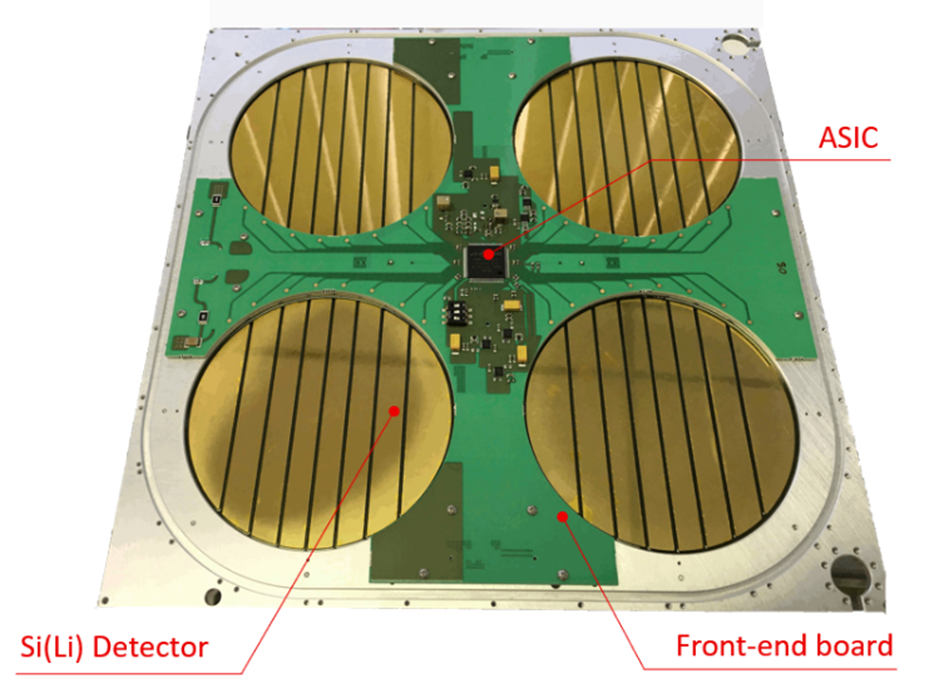
\includegraphics[height=0.4\textheight]{images/experiment_intro/GAPS_FEB_ASIC_3.png}
        \vspace{0.2cm}
        \vskip0.001cm
        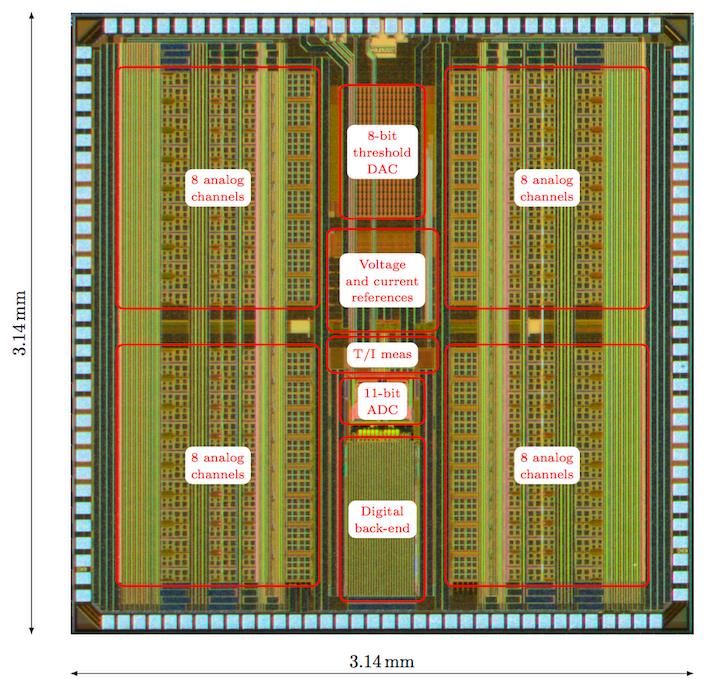
\includegraphics[height=0.35\textheight]{images/experiment_intro/gaps_asic_circuit.jpg}
        \end{figure}
    \end{columns}
\end{frame}
}

%----------------------------------------------------------------------------------------
%	Evaluation of temperature effects on ASIC performance
%----------------------------------------------------------------------------------------   

\section{Evaluation of temperature effects on ASIC performance}

\begin{frame}{Evaluation of temperature effects \\ \vskip-0.15cm on ASIC performance}
\fontsize{8.5pt}{1}\selectfont
    \begin{columns}[T]
    \column{0.475\textwidth}
        \vskip0.3cm
        \textbf{SLIDER32 ASIC test setup}\\
        \vskip0.15cm
        
        Tests conducted on the SLIDER32 readout ASIC with a purposely designed test board were aimed at evaluate temperature effects on:
        \begin{enumerate}
            \item Bandgap reference current
            \item Channel input-output characteristic
            \item DAC for setting the global threshold voltage
        \end{enumerate}

        \vskip0.05cm
        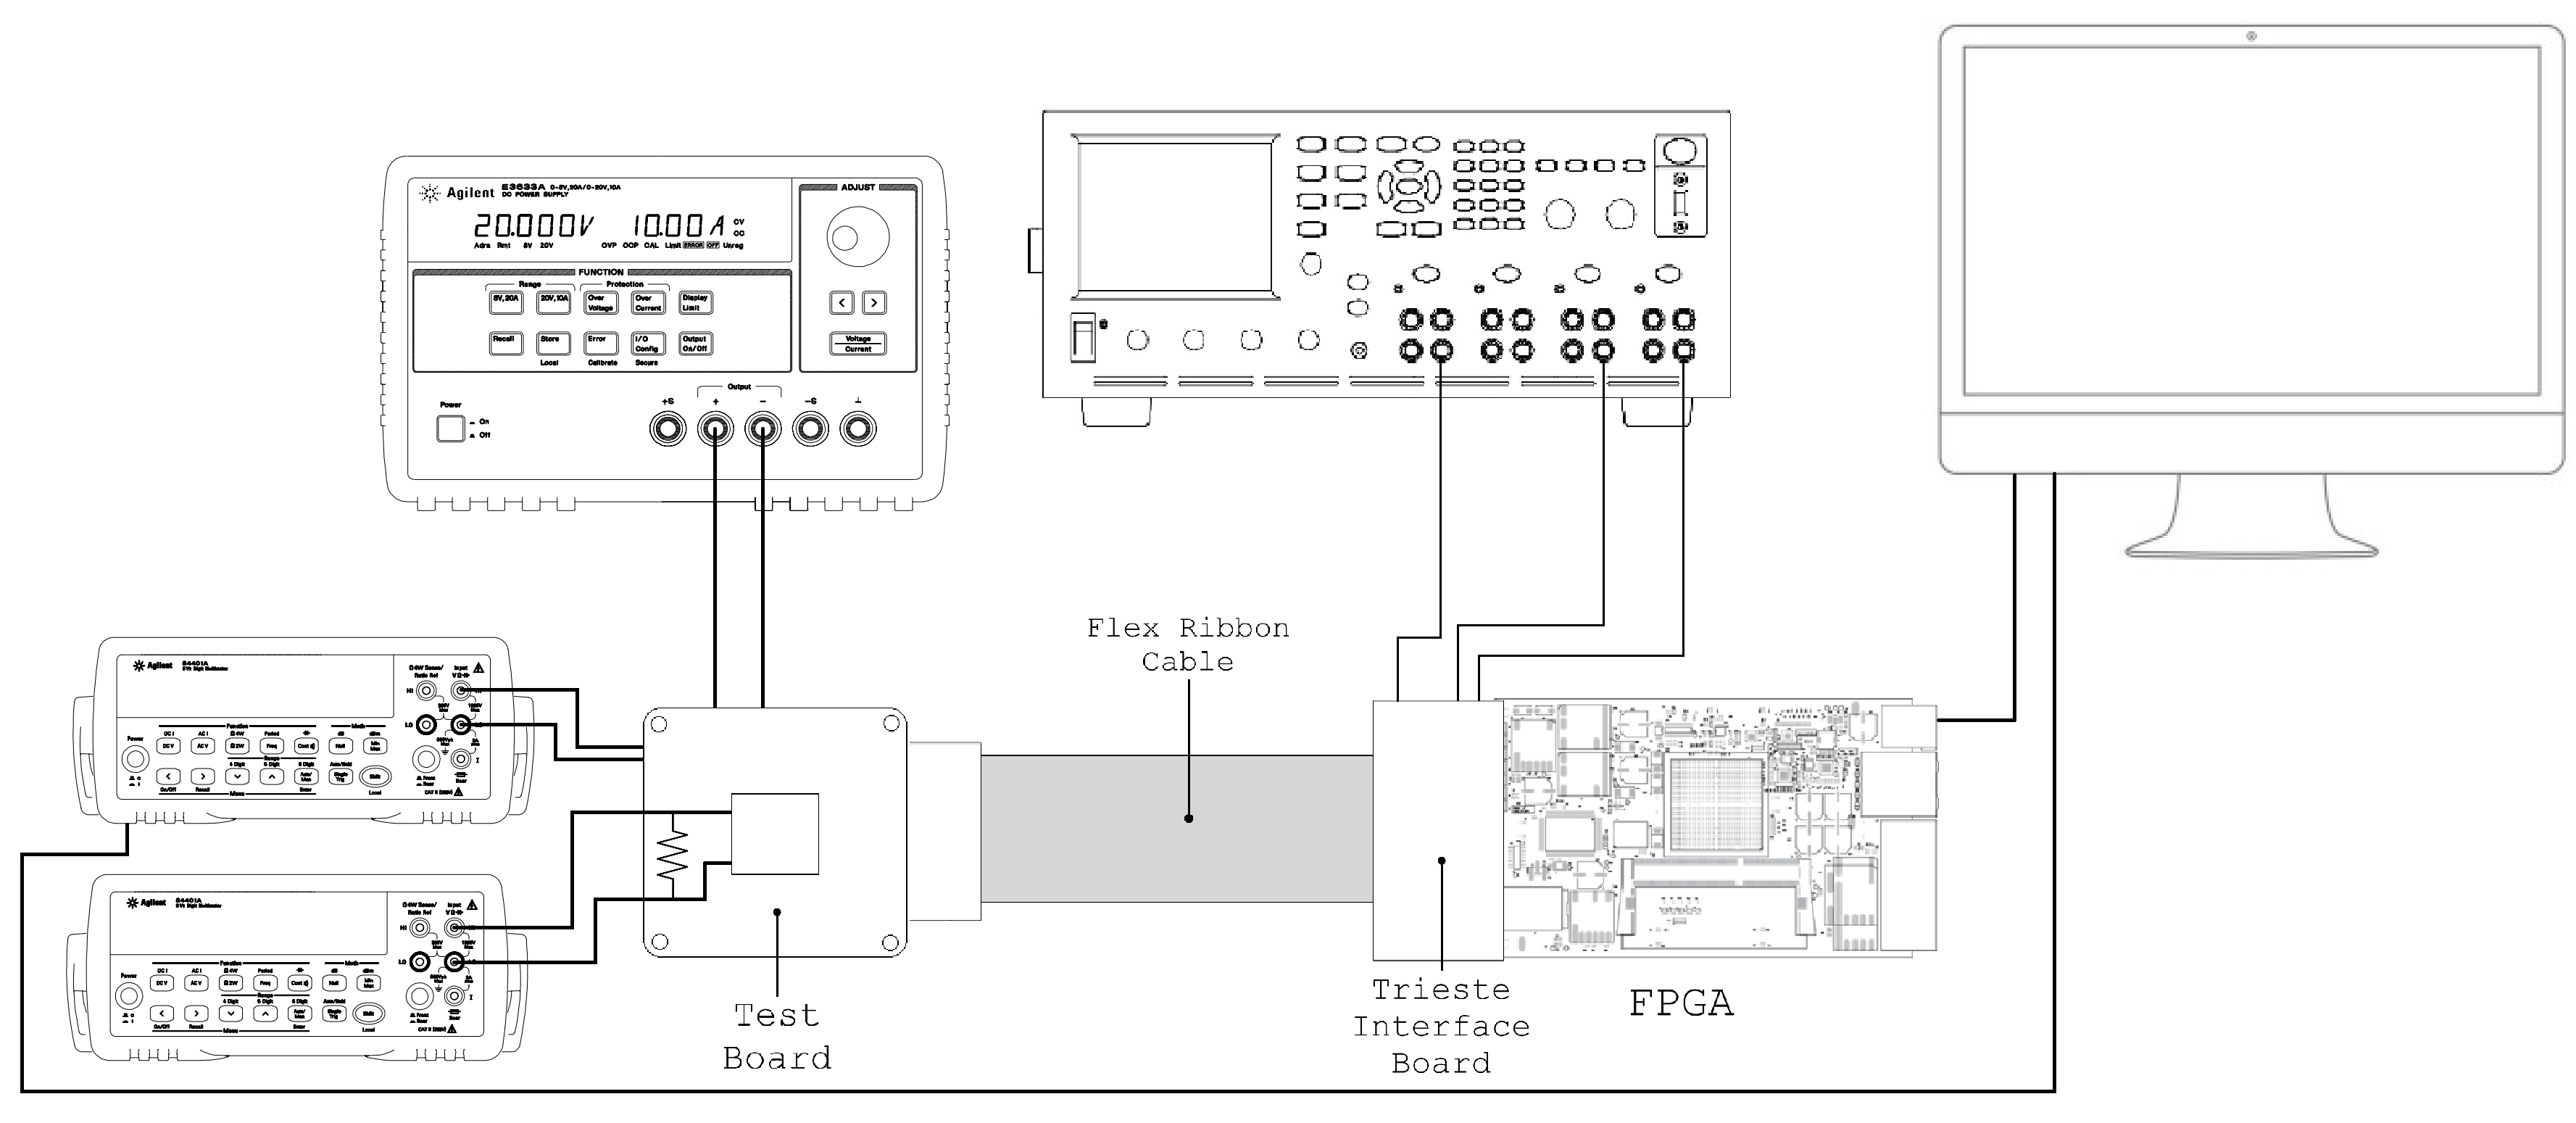
\includegraphics[width=0.95\textwidth]{images/temperature_effects/test_setup_test_board_csavrefgm_530mv.png}
        \vskip0.2cm

        Temperature range: 
        \begin{itemize}
            \item $\SI{-40}{\celsius} \div +\SI{30}{\celsius}$ with \SI{10}{\celsius} steps
            \item $\SI{-40}{\celsius} \div \SI{-30}{\celsius}$ with \SI{2}{\celsius} steps
        \end{itemize}
 
    \column{0.475\textwidth}
        \settowidth{\leftmargini}{\usebeamertemplate{itemize item}}
        \addtolength{\leftmargini}{\labelsep}
        \vskip0.3cm
        \textbf{Bandgap reference current}\\
        \vskip0.15cm
    
        Adjustable current reference by means of 3 bits (\texttt{BBB}) and \SI{5}{\micro\ampere} nominal value

        \vskip-0.4cm
        \begin{center}
            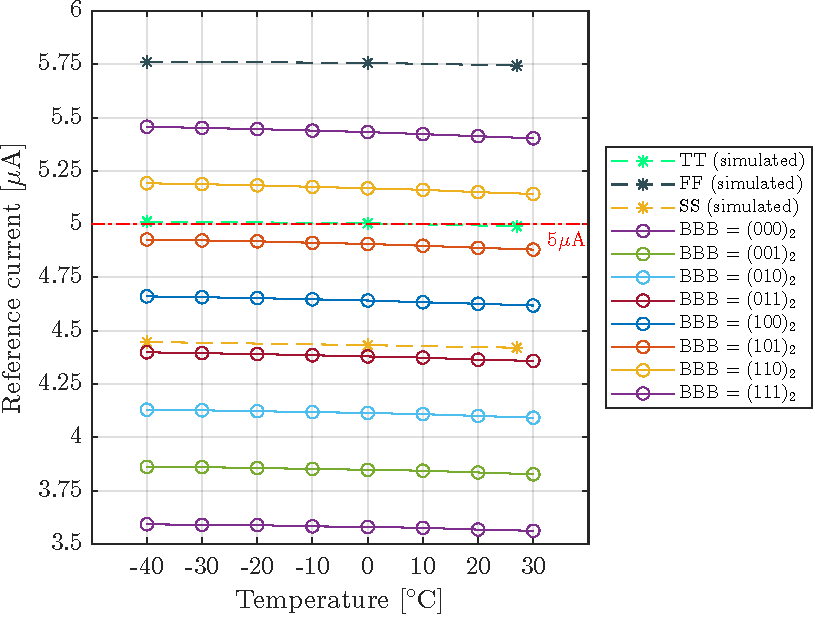
\includegraphics[height=0.48\textheight]{images/temperature_effects/BGR_current_Xtemp_all-BBB.pdf}
        \end{center}

        \vskip-0.2cm
        \begin{itemize}
            \item \SI{5}{\micro\ampere} nominal value obtained with \texttt{BBB} = $(\texttt{101})_{2}$ \greencheck
            \item $< \SI{1}{\percent}$ variation over the whole temperature range \greencheck
            \item $\thicksim \SI{1.8}{\micro\ampere}$ range @ \SI{-40}{\celsius} by adjusting \texttt{BBB} bits \greencheck
        \end{itemize}
    
    \end{columns}
\end{frame}

{\singlelinelogo
\begin{frame}{Channel input-output characteristic}
\fontsize{8.5pt}{1}\selectfont
    \begin{columns}[T]
    \column{0.475\textwidth}
        \settowidth{\leftmargini}{\usebeamertemplate{itemize item}}
        \addtolength{\leftmargini}{\labelsep}
        \vskip0.3cm
        \textbf{Automatically regulated \texttt{CSAVrefGM} voltage}\\
        \vskip0.15cm
    
        txt

        \vskip-0.4cm
        \begin{center}
            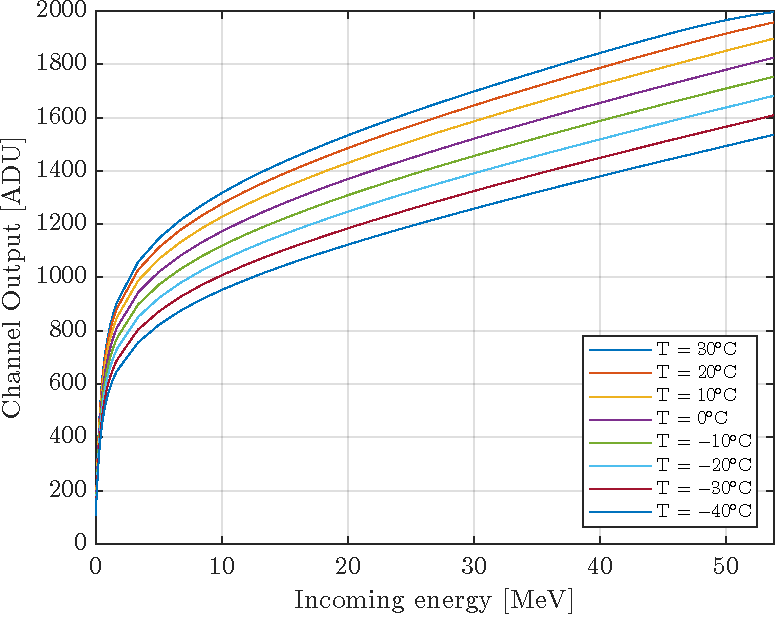
\includegraphics[height=0.48\textheight]{images/temperature_effects/fdt_csavrefgm_auto_tau6_keV_0011.pdf}
        \end{center}

        \vskip-0.2cm
        \begin{itemize}
            \item txt
        \end{itemize}

        \column{0.475\textwidth}
            \settowidth{\leftmargini}{\usebeamertemplate{itemize item}}
            \addtolength{\leftmargini}{\labelsep}
            \vskip0.3cm
            \textbf{\texttt{CSAVrefGM} voltage set to \SI{530}{\milli\volt}}\\
            \vskip0.15cm
        
            txt
    
            \vskip-0.4cm
            \begin{center}
                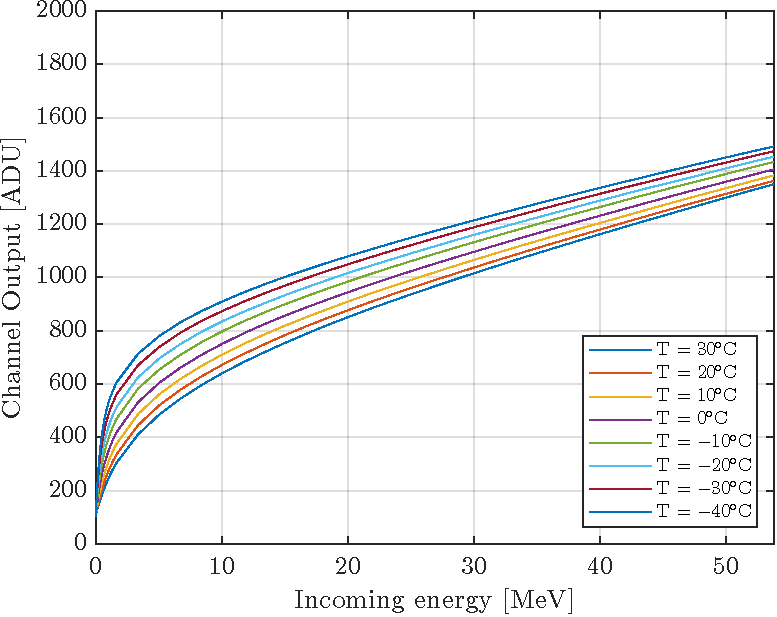
\includegraphics[height=0.48\textheight]{images/temperature_effects/fdt_csavrefgm_530mV_tau6_keV.pdf}
            \end{center}
    
            \vskip-0.2cm
            \begin{itemize}
                \item txt
            \end{itemize}
    
    \end{columns}
\end{frame}
}


\begin{frame}{Kink trend as function of temperature}
\fontsize{8.5pt}{1}\selectfont
    \begin{columns}[T]
    \column{0.475\textwidth}
        \settowidth{\leftmargini}{\usebeamertemplate{itemize item}}
        \addtolength{\leftmargini}{\labelsep}
        \vskip0.3cm
        \textbf{Automatically regulated \texttt{CSAVrefGM} voltage}\\
        \vskip0.15cm
    
        txt

        \vskip-0.4cm
        \begin{center}
            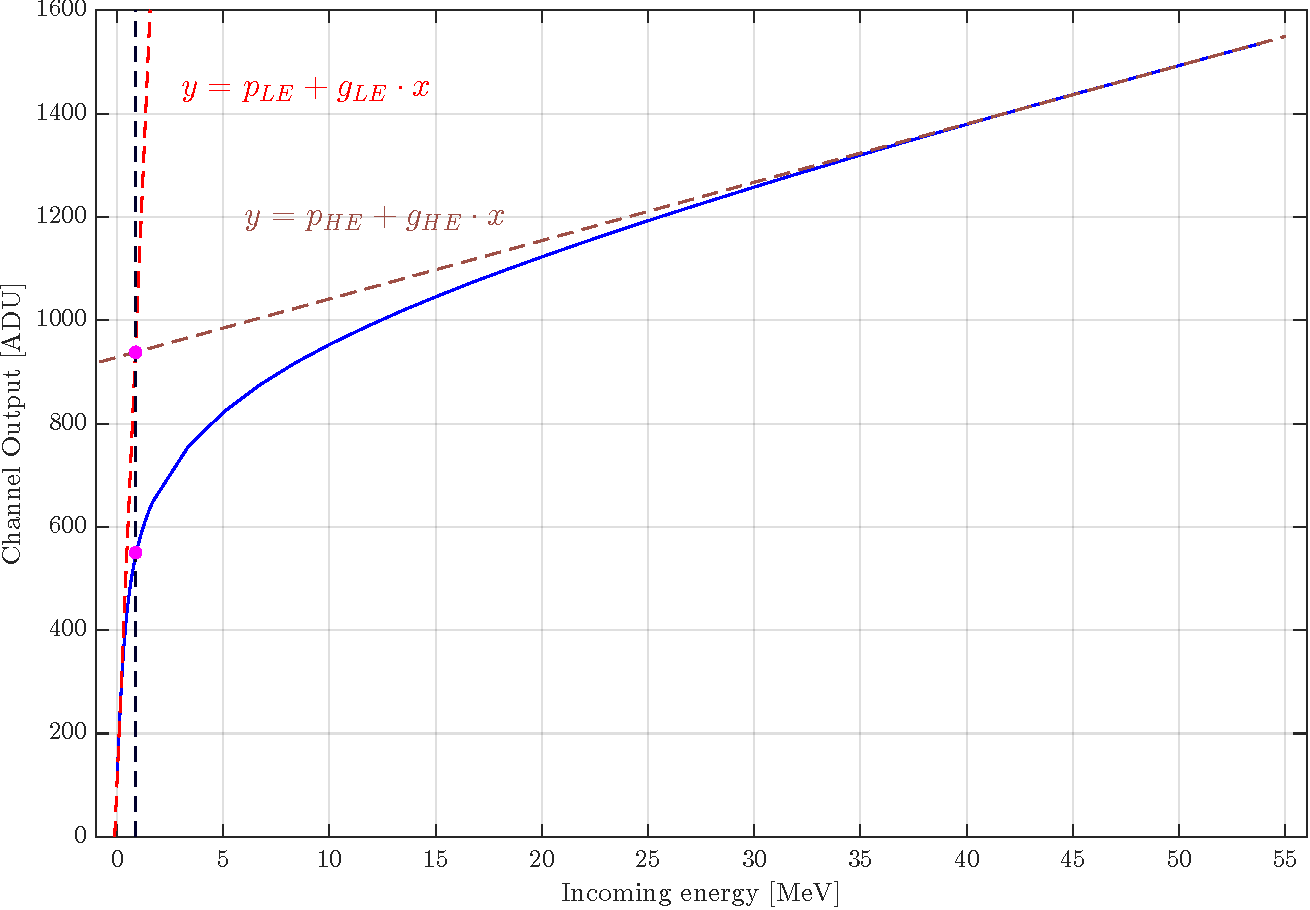
\includegraphics[height=0.48\textheight]{images/temperature_effects/fdt_calcolo_kink.pdf}
        \end{center}

        \vskip-0.2cm
        \begin{itemize}
            \item txt
        \end{itemize}

        \column{0.475\textwidth}
            \settowidth{\leftmargini}{\usebeamertemplate{itemize item}}
            \addtolength{\leftmargini}{\labelsep}
            \vskip0.3cm
            \textbf{\texttt{CSAVrefGM} voltage set to \SI{530}{\milli\volt}}\\
            \vskip0.15cm
        
            txt
    
            \vskip-0.4cm
            \begin{center}
                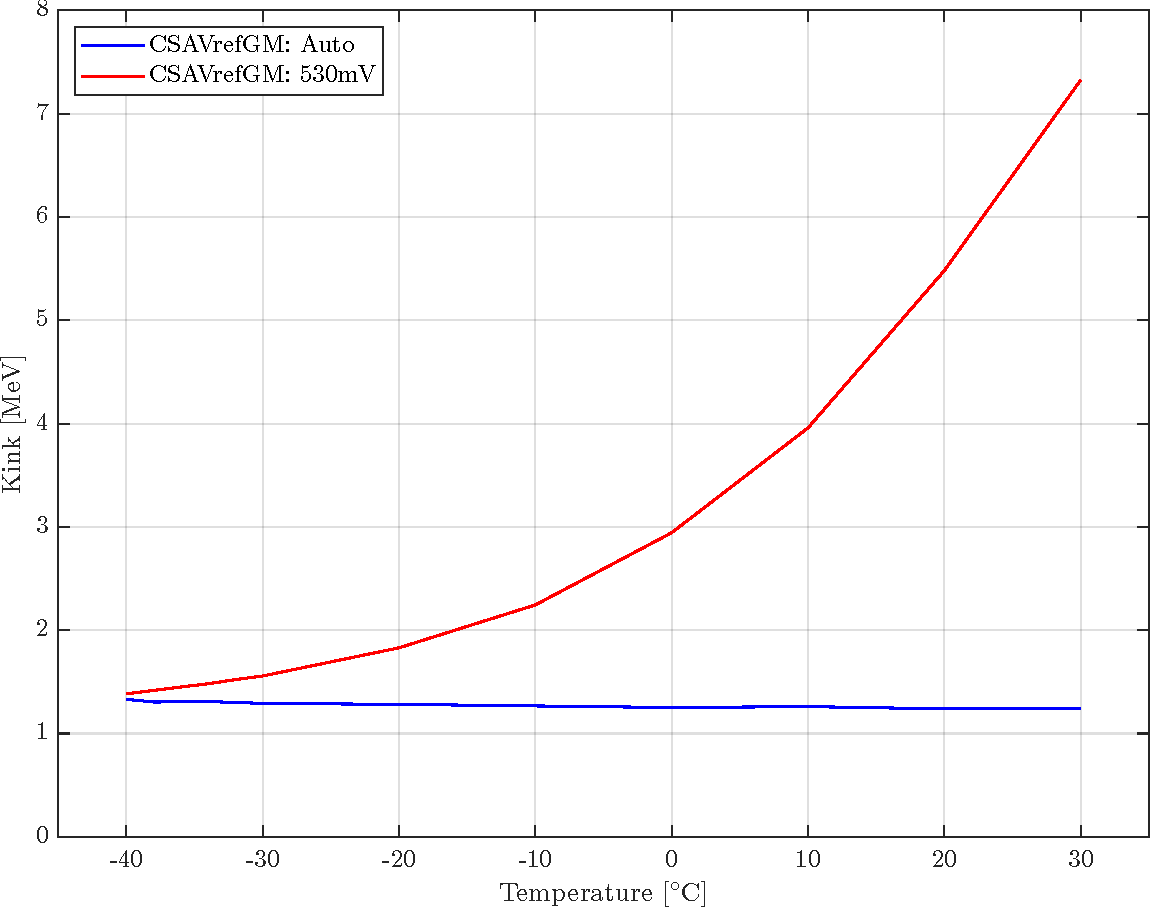
\includegraphics[height=0.48\textheight]{images/temperature_effects/plot_pedestal_gain_auto_530mV.pdf}
            \end{center}
    
            \vskip-0.2cm
            \begin{itemize}
                \item txt
            \end{itemize}
    
    \end{columns}
\end{frame}


\begin{frame}{DAC for setting the global\\ \vskip-0.15cm threshold voltage}
\fontsize{8.5pt}{1}\selectfont
    \begin{columns}[T]
    \column{0.475\textwidth}
        \settowidth{\leftmargini}{\usebeamertemplate{itemize item}}
        \addtolength{\leftmargini}{\labelsep}
        \vskip0.3cm
        \textbf{Automatically regulated \texttt{CSAVrefGM} voltage}\\
        \vskip0.15cm
    
        txt

        \vskip-0.4cm
        \begin{center}
            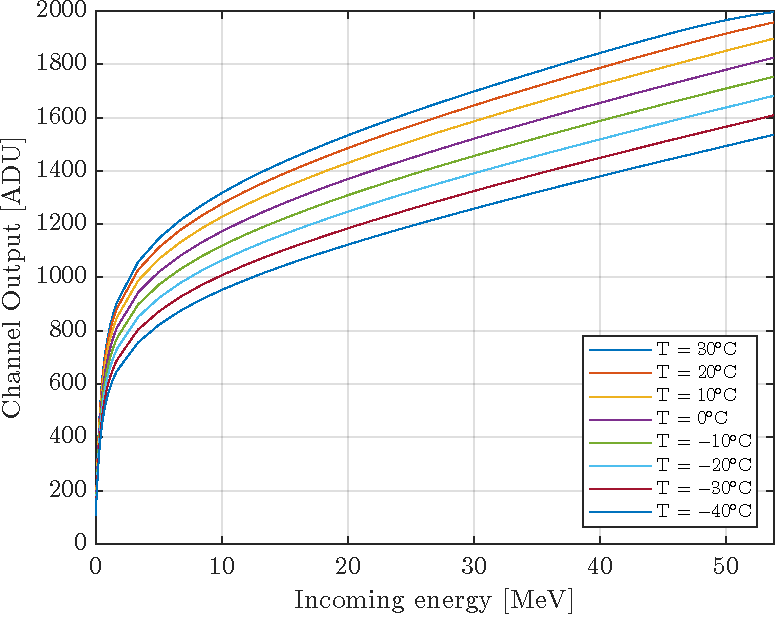
\includegraphics[height=0.48\textheight]{images/temperature_effects/fdt_csavrefgm_auto_tau6_keV_0011.pdf}
        \end{center}

        \vskip-0.2cm
        \begin{itemize}
            \item txt
        \end{itemize}

        \column{0.475\textwidth}
            \settowidth{\leftmargini}{\usebeamertemplate{itemize item}}
            \addtolength{\leftmargini}{\labelsep}
            \vskip0.3cm
            \textbf{\texttt{CSAVrefGM} voltage set to \SI{530}{\milli\volt}}\\
            \vskip0.15cm
        
            txt
    
            \vskip-0.4cm
            \begin{center}
                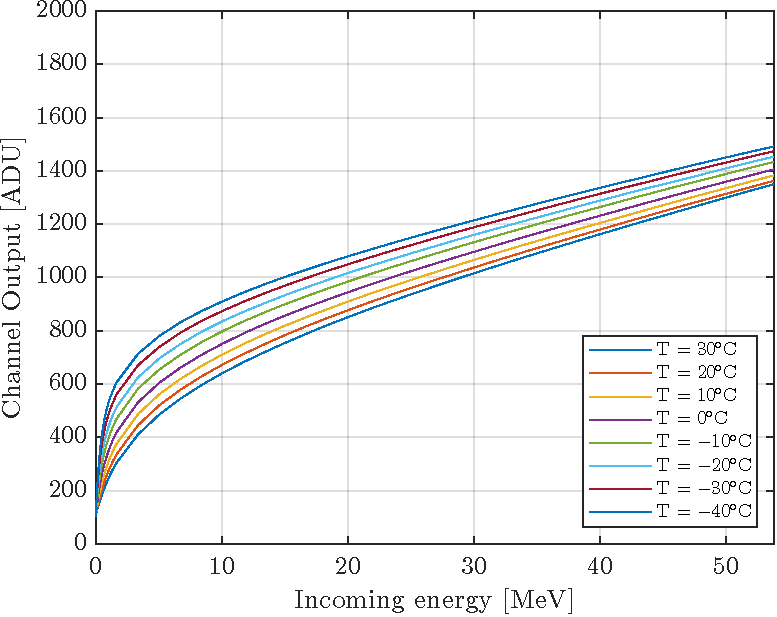
\includegraphics[height=0.48\textheight]{images/temperature_effects/fdt_csavrefgm_530mV_tau6_keV.pdf}
            \end{center}
    
            \vskip-0.2cm
            \begin{itemize}
                \item txt
            \end{itemize}
    
    \end{columns}
\end{frame}


%----------------------------------------------------------------------------------------
%	Si(Li) tracker flight components validation
%----------------------------------------------------------------------------------------

\section{Si(Li) tracker flight components validation}

\subsection{Front-End Board (FEB)}
\begin{frame}{\vspace{-0.3cm}Si(Li) tracker flight components \\ \vskip-0.15cm validation}
    \fontsize{9pt}{1}\selectfont
    \vskip0.15cm
    \textbf{\large Front-End Board (FEB)} \\
    \vspace{0.15cm}
    The test of the front-end boards has been performed at ambient temperature and was aimed at verifying the proper functioning of the board and at looking for damages to the board or improperly soldered components.

    \vskip0.3cm
    \begin{columns}[T]
        \column{0.3\textwidth}
            \begin{figure}
                \centering
                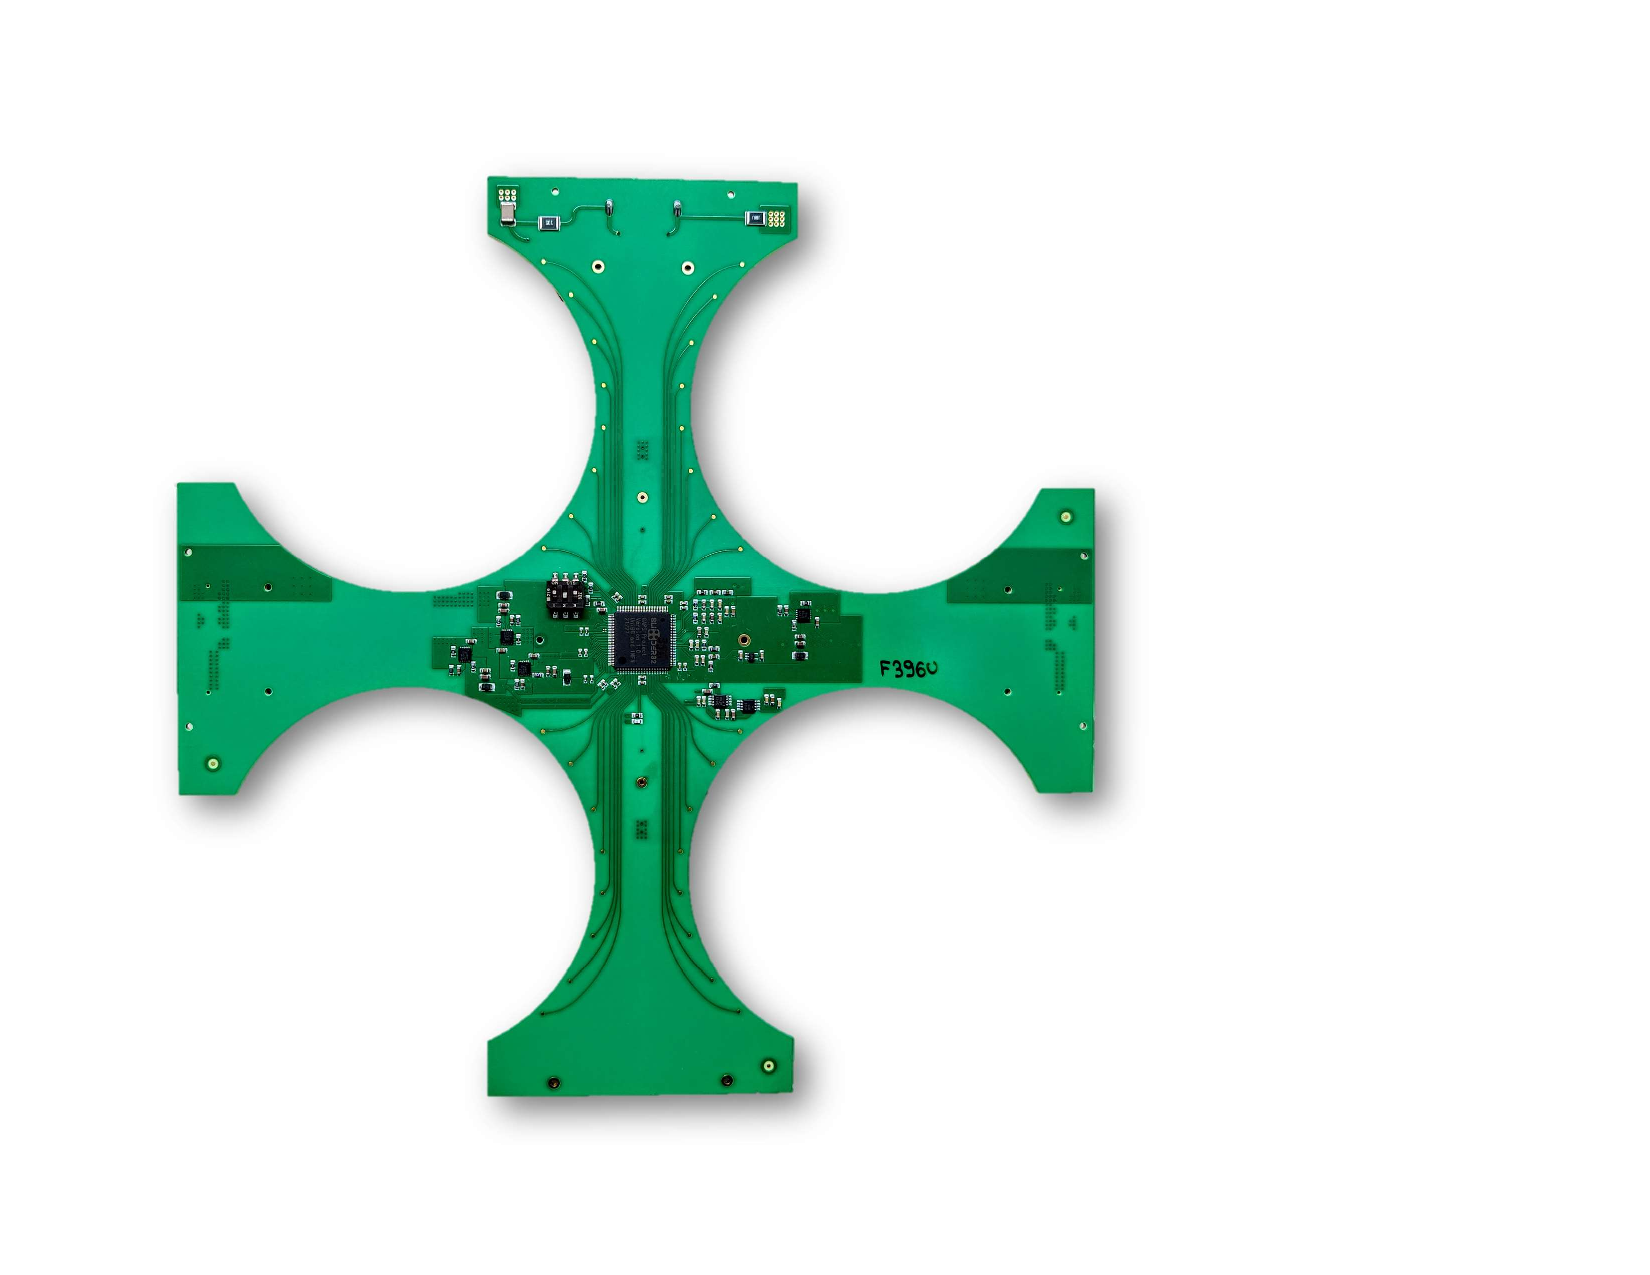
\includegraphics[width=0.9\textwidth]{images/flight_components_validation/FEB_immagine.pdf}
            \end{figure}
        
        \column{0.7\textwidth}
            \begin{figure}
                \centering
                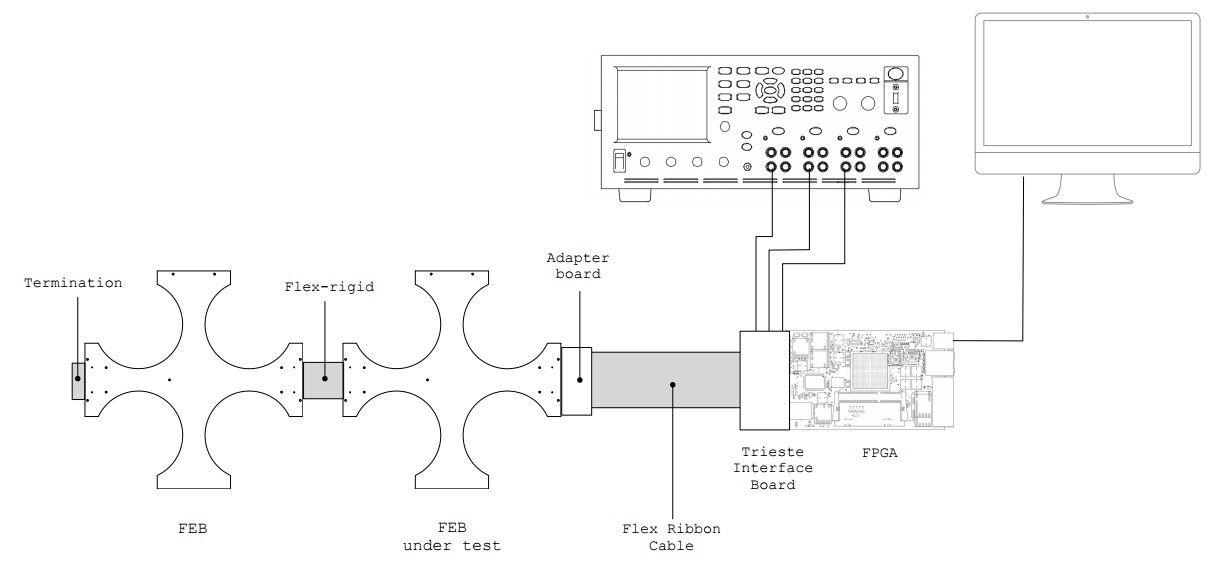
\includegraphics[width=0.8\textwidth]{images/flight_components_validation/test_setup_FEB_2.jpg}
            \end{figure}
            txt here
    \end{columns}
\end{frame}

{\singlelinelogo
\begin{frame}{Front-End Board: test results}
    \fontsize{9pt}{1}\selectfont
    \vskip0.15cm

\end{frame}
}

\subsection{Dummy-1 Front-End Board}
{\singlelinelogo
\begin{frame}{Dummy-1 Front-End Board}
    \fontsize{9pt}{1}\selectfont
    \vskip0.15cm

\end{frame}
}

\subsection{Other flight components}
{\singlelinelogo
\begin{frame}{Other flight components}
    \fontsize{9pt}{1}\selectfont
    \vskip0.15cm

\end{frame}
}

%----------------------------------------------------------------------------------------
%	Muon detection using an assembled Si(Li) tracker module
%----------------------------------------------------------------------------------------

\section{Experimental results from module test}

\begin{frame}{\vspace{-0.3cm}Experimental results from\\ \vskip-0.15cm module test}
    \settowidth{\leftmargini}{\usebeamertemplate{itemize item}}
    \addtolength{\leftmargini}{\labelsep}

    \begin{columns}
        \column{0.63\textwidth}

            \fontsize{10pt}{1}\selectfont
            \vskip0.1cm
            \textbf{Si(Li) tracker module test setup} \\
            \vspace{0.05cm}
            
            \fontsize{8.5pt}{1}\selectfont
            \begin{itemize}
                \item Tests performed in a climatic chamber at \SI{-40}{\celsius} and \SI{10}{\percent} humidity
                \item Peaking time \#4 ($\tau_{p} = \SI{0.98}{\micro\second}$)
                \item Self-Trigger mode employed
                \item 1 hour long acquisition
            \end{itemize}
            
            \begin{columns}
                \column{0.6\textwidth}
                    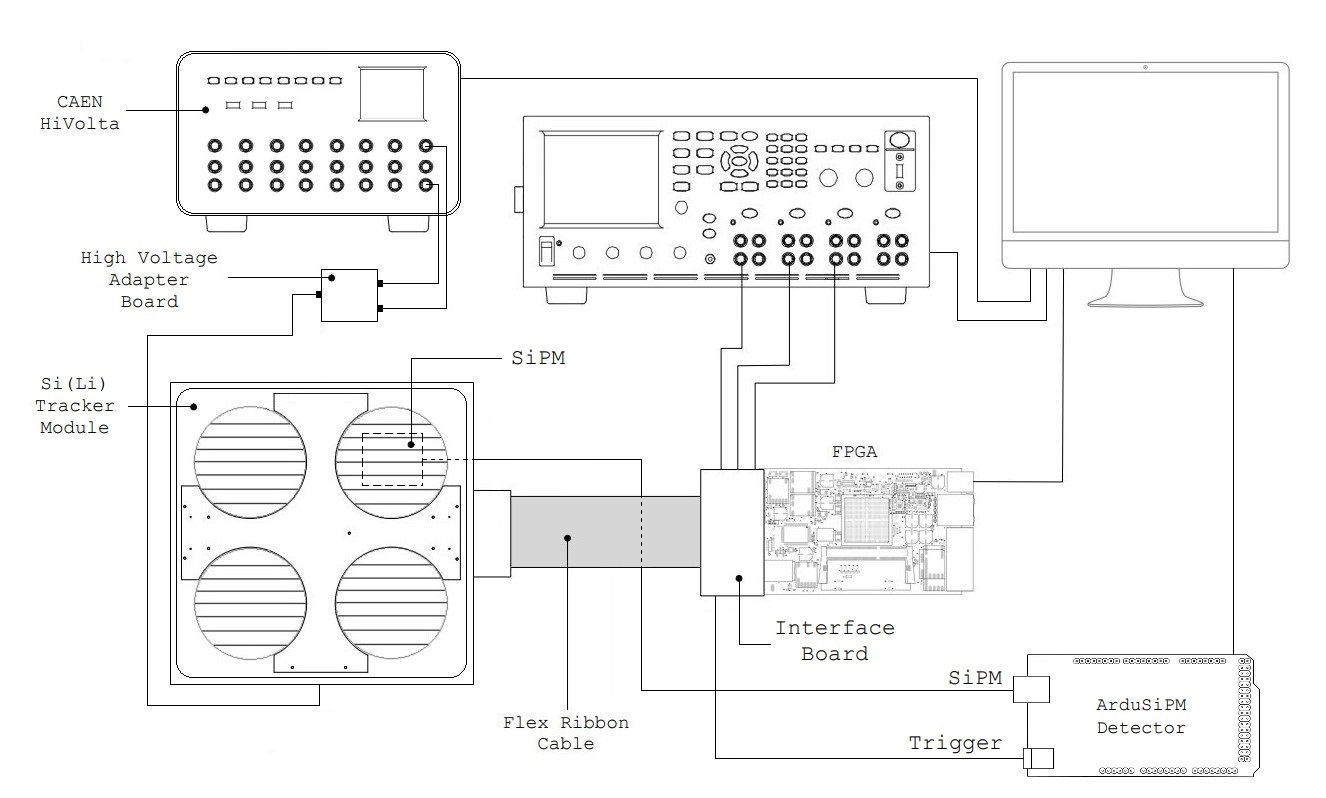
\includegraphics[width=0.99\textwidth]{images/muon_detection/test_setup_MODULE.jpg}
                \column{0.4\textwidth}
                    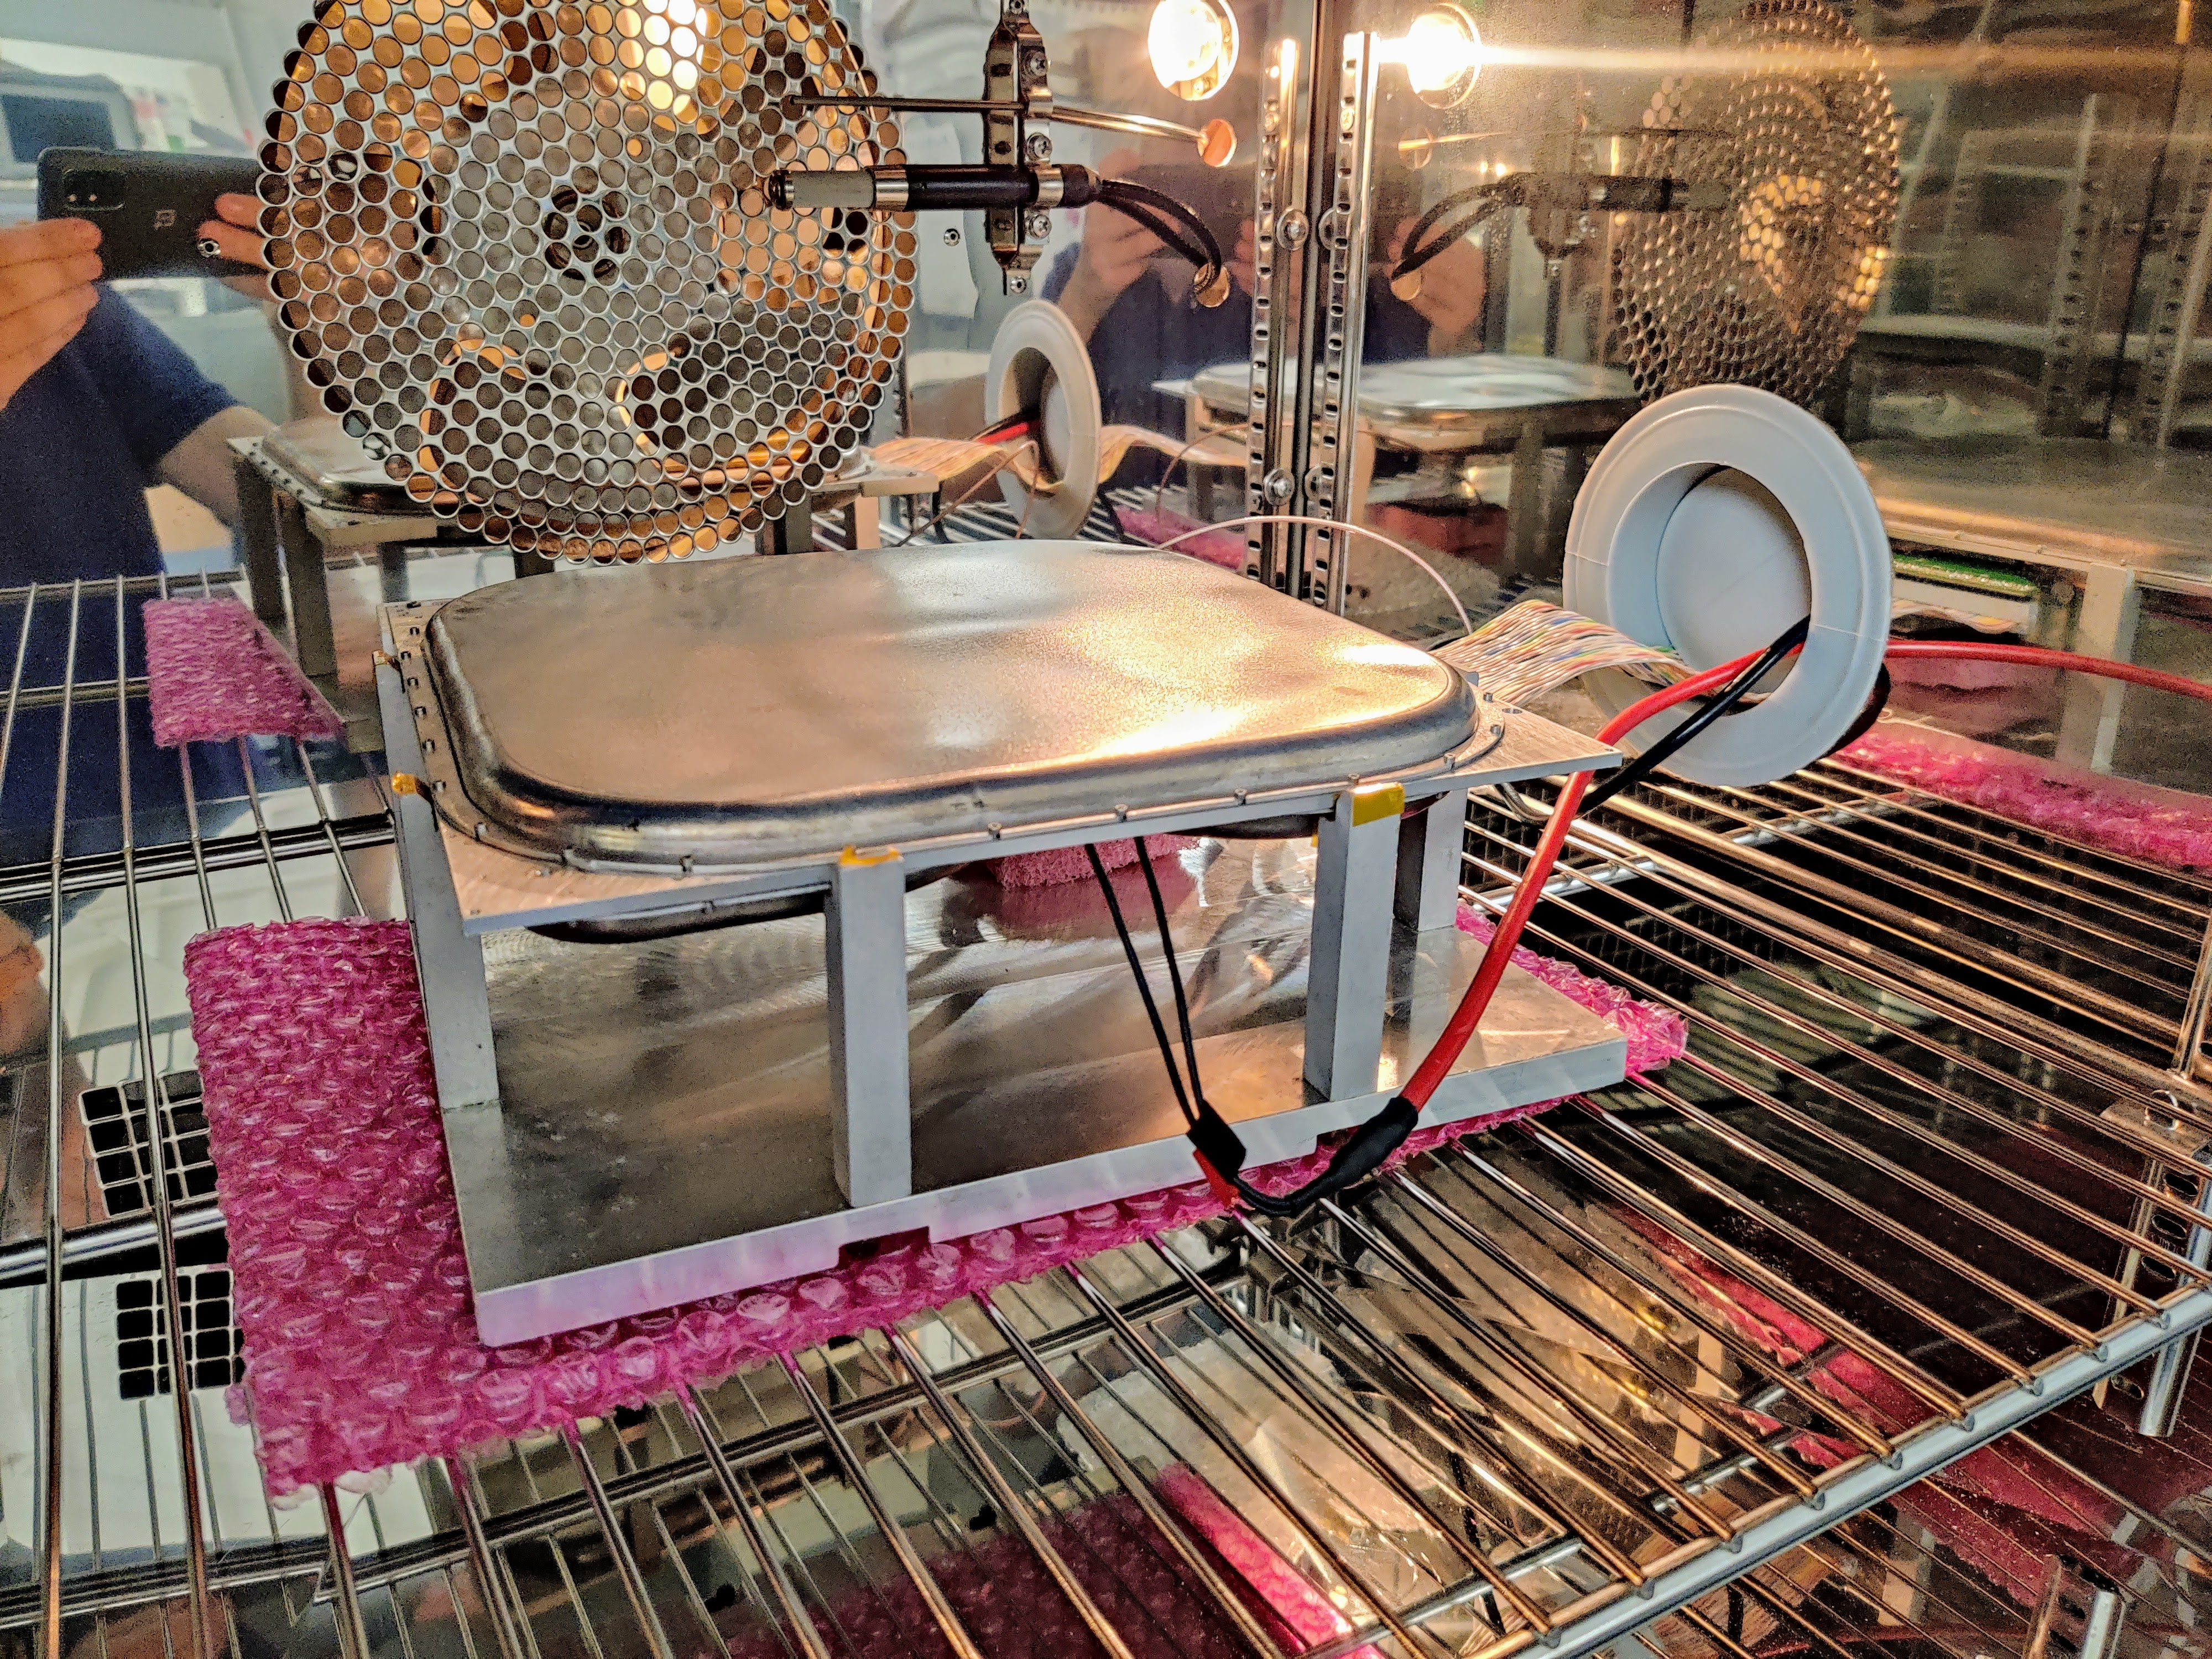
\includegraphics[width=0.9\textwidth]{images/muon_detection/foto_modulo_camera.jpg}
            \end{columns}

            \fontsize{10pt}{1}\selectfont
            \textbf{Results} \\
            \vspace{0.05cm}

            \fontsize{8.5pt}{1}\selectfont
            \begin{itemize}
                \item \SI{59.54}{\kilo\electronvolt} and \SI{26.34}{\kilo\electronvolt} \ce{^{241}Am} $\gamma$ emission peaks detected with visible \textit{Compton Shoulder} \greencheck
                \item Self-Trigger and Zero Suppression modes correctly tested \greencheck
            \end{itemize}

        \column{0.32\textwidth}
            \fontsize{7pt}{1}\selectfont
            \centering
            \textbf{\ce{^{241}Am} source detection} \\
            \vspace{0.1cm}
            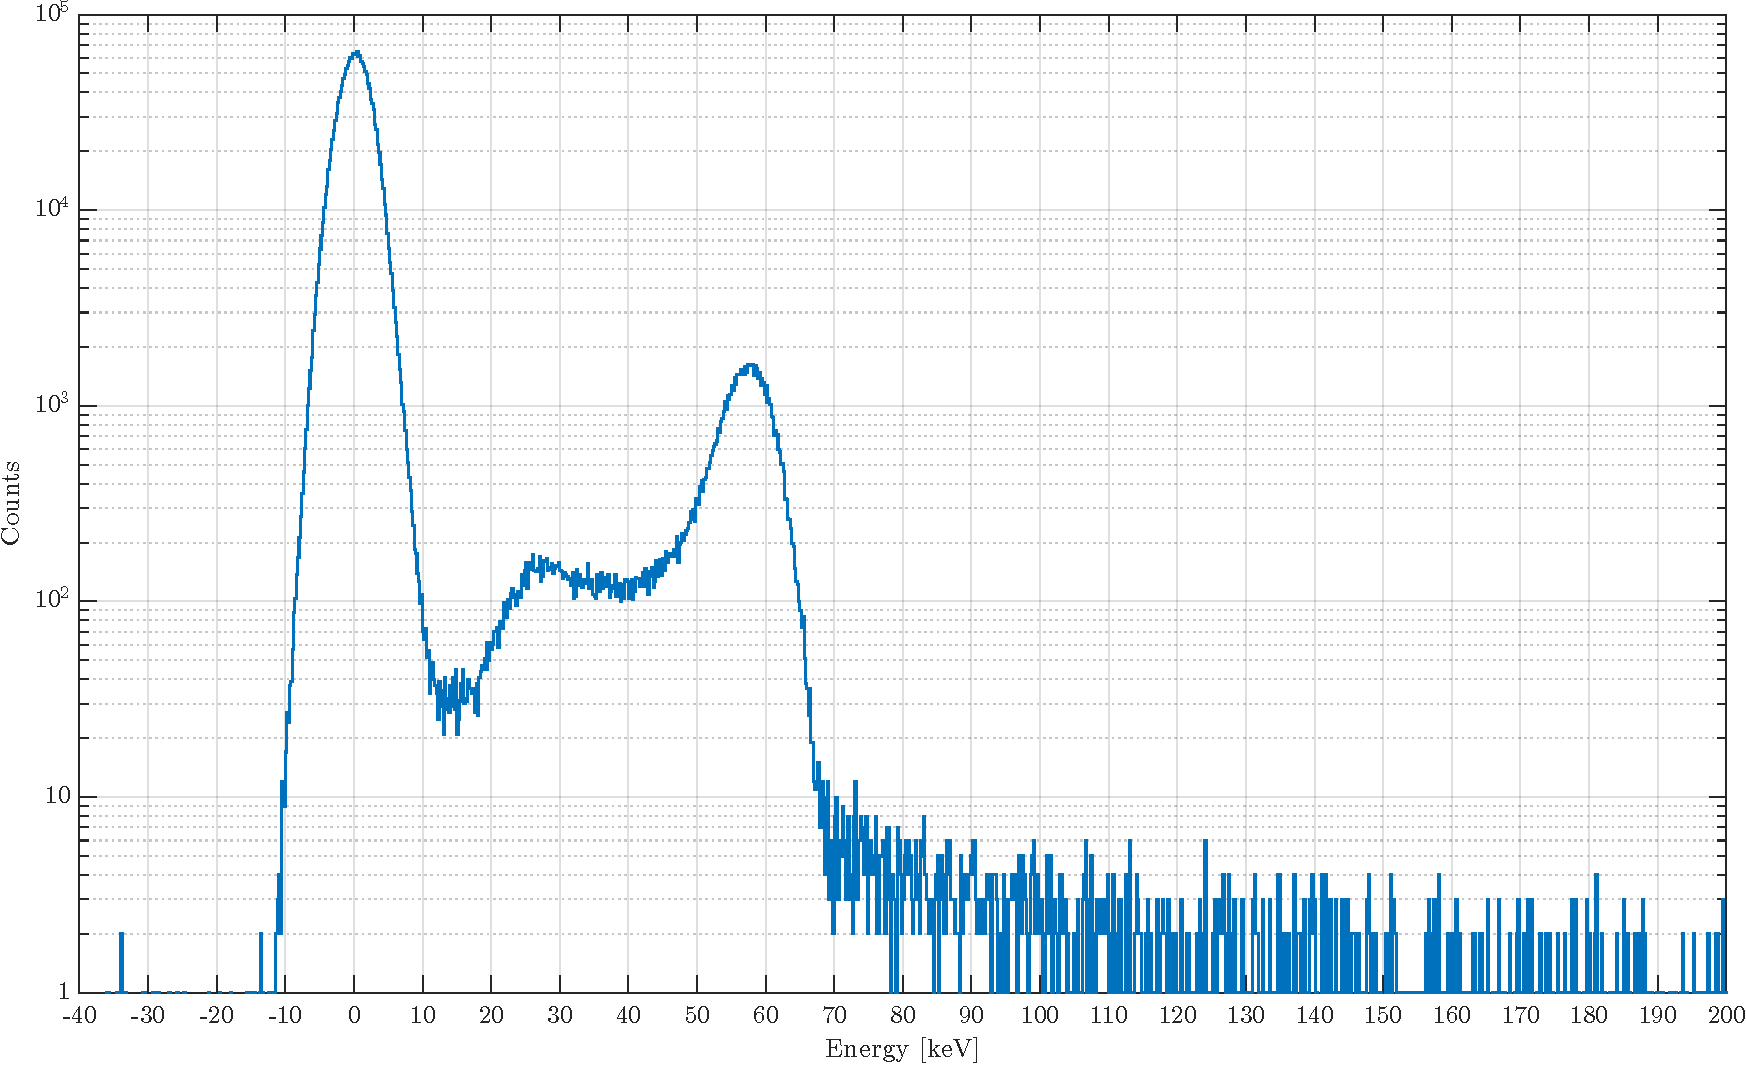
\includegraphics[width=0.99\textwidth]{images/muon_detection/ch4_americio_log.pdf}
            
            \vskip0.15cm
            \textbf{Cosmic muon detection} \\
            \vspace{0.1cm}
            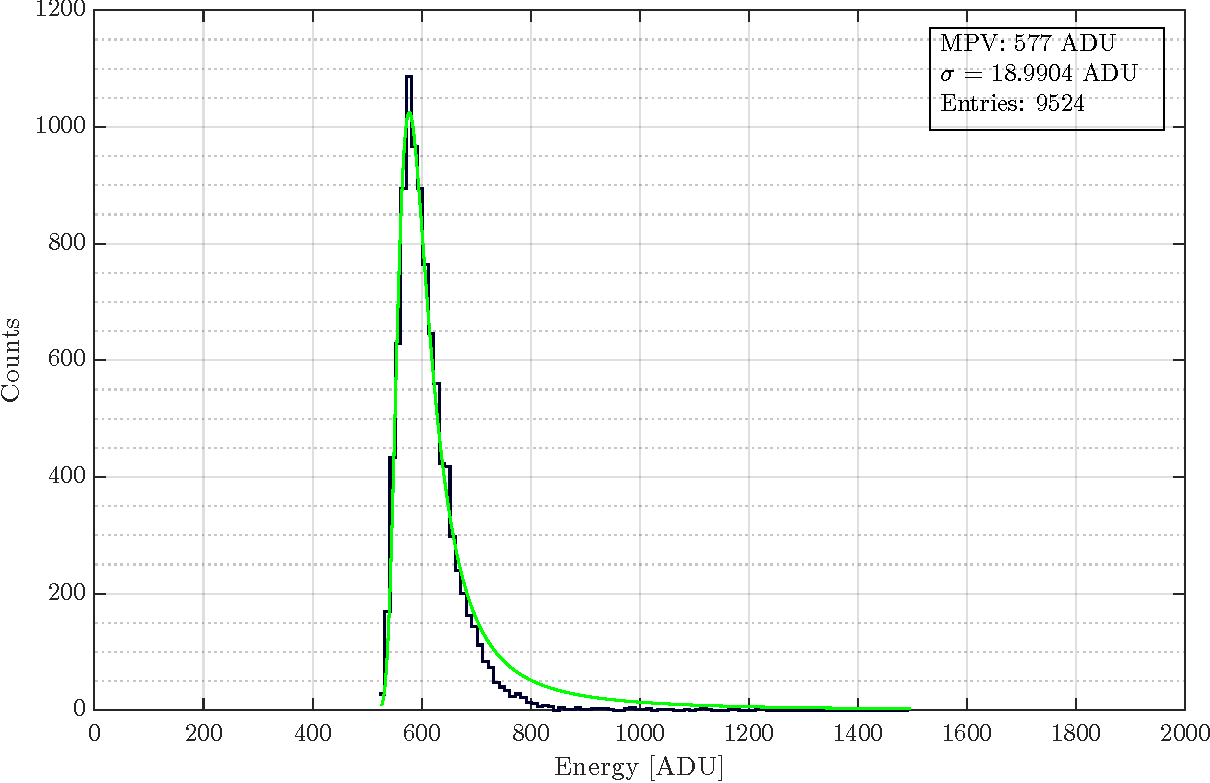
\includegraphics[width=0.99\textwidth]{images/muon_detection/incoming_energy_thr130_ZS_landau.pdf}
    \end{columns}
\end{frame}

\begin{frame}{\vspace{-0.3cm} Cosmic muon detection in\\ \vskip-0.15cm external trigger mode}
    \settowidth{\leftmargini}{\usebeamertemplate{itemize item}}
    \addtolength{\leftmargini}{\labelsep}
    \fontsize{9pt}{1}\selectfont

    \begin{columns}
        \column{0.33\textwidth}
        \begin{itemize}
            \item Scintillator/SiPM assembly placed underneath Si(Li) detector \#2: channels 16 to 23 highlighted in red

            \vskip0.4cm
            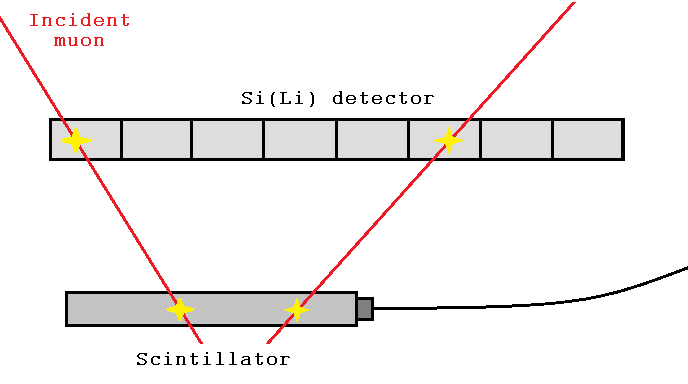
\includegraphics[width=0.9\textwidth]{images/muon_detection/scintillator_sensor_detail.png}

            \vskip0.4cm
            \item \textit{ArduSiPM} device used as an external trigger source
            \item 2 hours long acquisition
            \item Global threshold set to \texttt{130}
            \item Trigger hold delay set to \texttt{34} FPGA clocks
            
        \end{itemize}

        \column{0.65\textwidth}
            \vskip-0.2cm
            \begin{figure}[h!]
                \centering
                \begin{tabular}{c c}
                    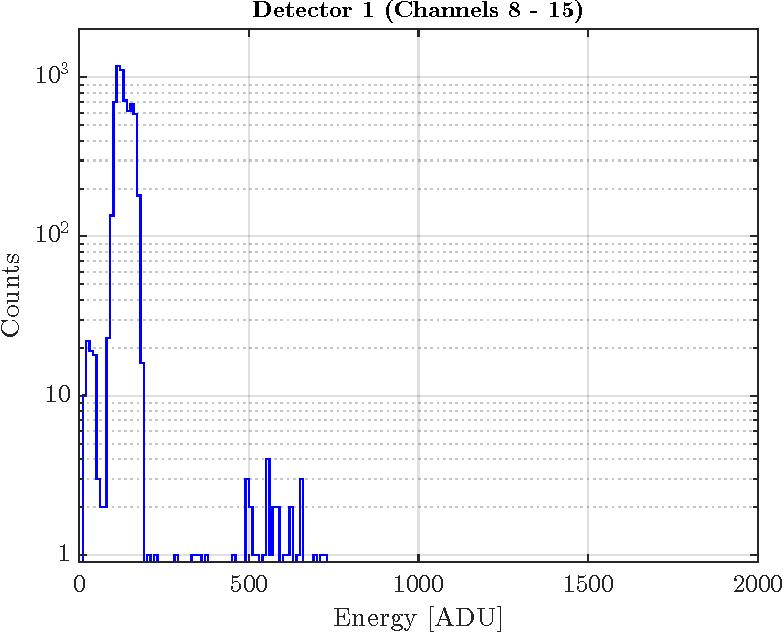
\includegraphics[width=0.44\textwidth]{images/muon_detection/incoming_energy34_2hr_sens2.pdf} & 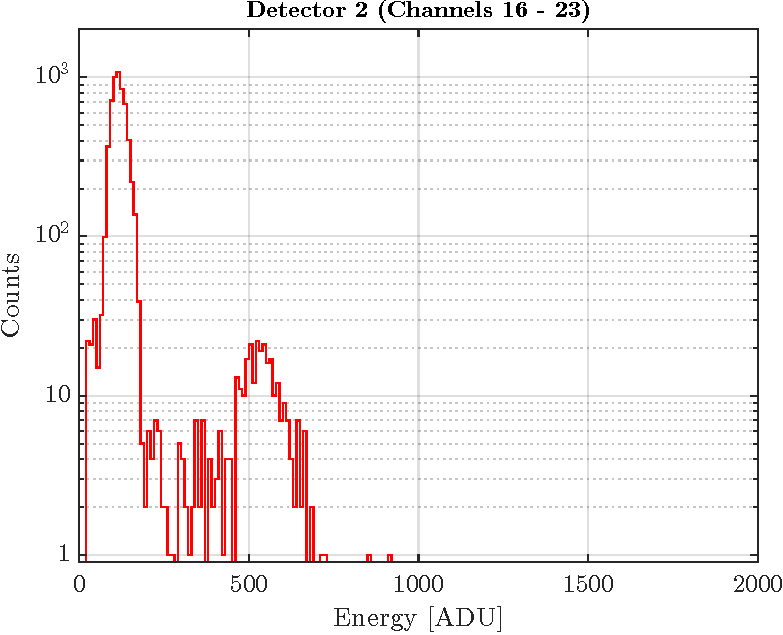
\includegraphics[width=0.44\textwidth]{images/muon_detection/incoming_energy34_2hr_sens3.pdf}\B \\
                    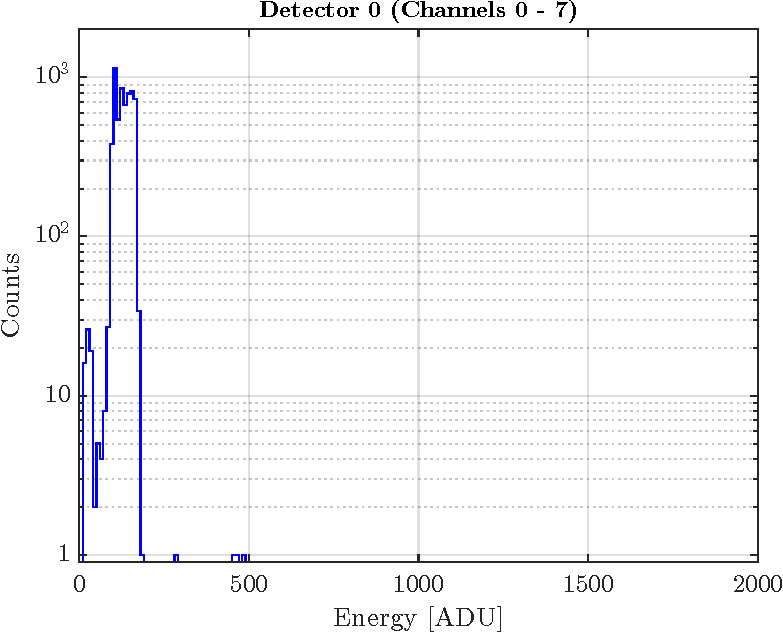
\includegraphics[width=0.44\textwidth]{images/muon_detection/incoming_energy34_2hr_sens1.pdf} & 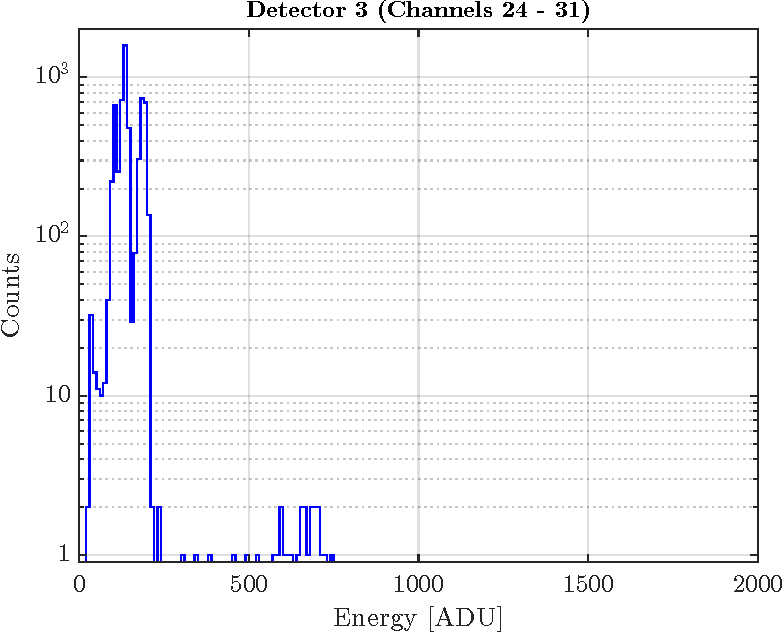
\includegraphics[width=0.44\textwidth]{images/muon_detection/incoming_energy34_2hr_sens4.pdf}
                \end{tabular}
            \end{figure}
        
    \end{columns}
    
\end{frame}

%----------------------------------------------------------------------------------------
%	Conclusions
%----------------------------------------------------------------------------------------

\section{Conclusions}

{\singlelinelogo
\begin{frame}{Conclusions}
    txt
\end{frame}
}

%----------------------------------------------------------------------------------------
%	Backup slides
%----------------------------------------------------------------------------------------

\appendix
\backupbegin

{\sectiontitlelogo
\begin{frame}{}
    \fontsize{19pt}{1}\selectfont
    \centering
    \vspace{1.5cm}
    \textbf{Backup slides}
\end{frame}
}

{\singlelinelogo
\begin{frame}{Analog readout channel and ADC}
    \fontsize{8.5pt}{1}\selectfont
    \settowidth{\leftmargini}{\usebeamertemplate{itemize item}}
    \addtolength{\leftmargini}{\labelsep}
    \centering
    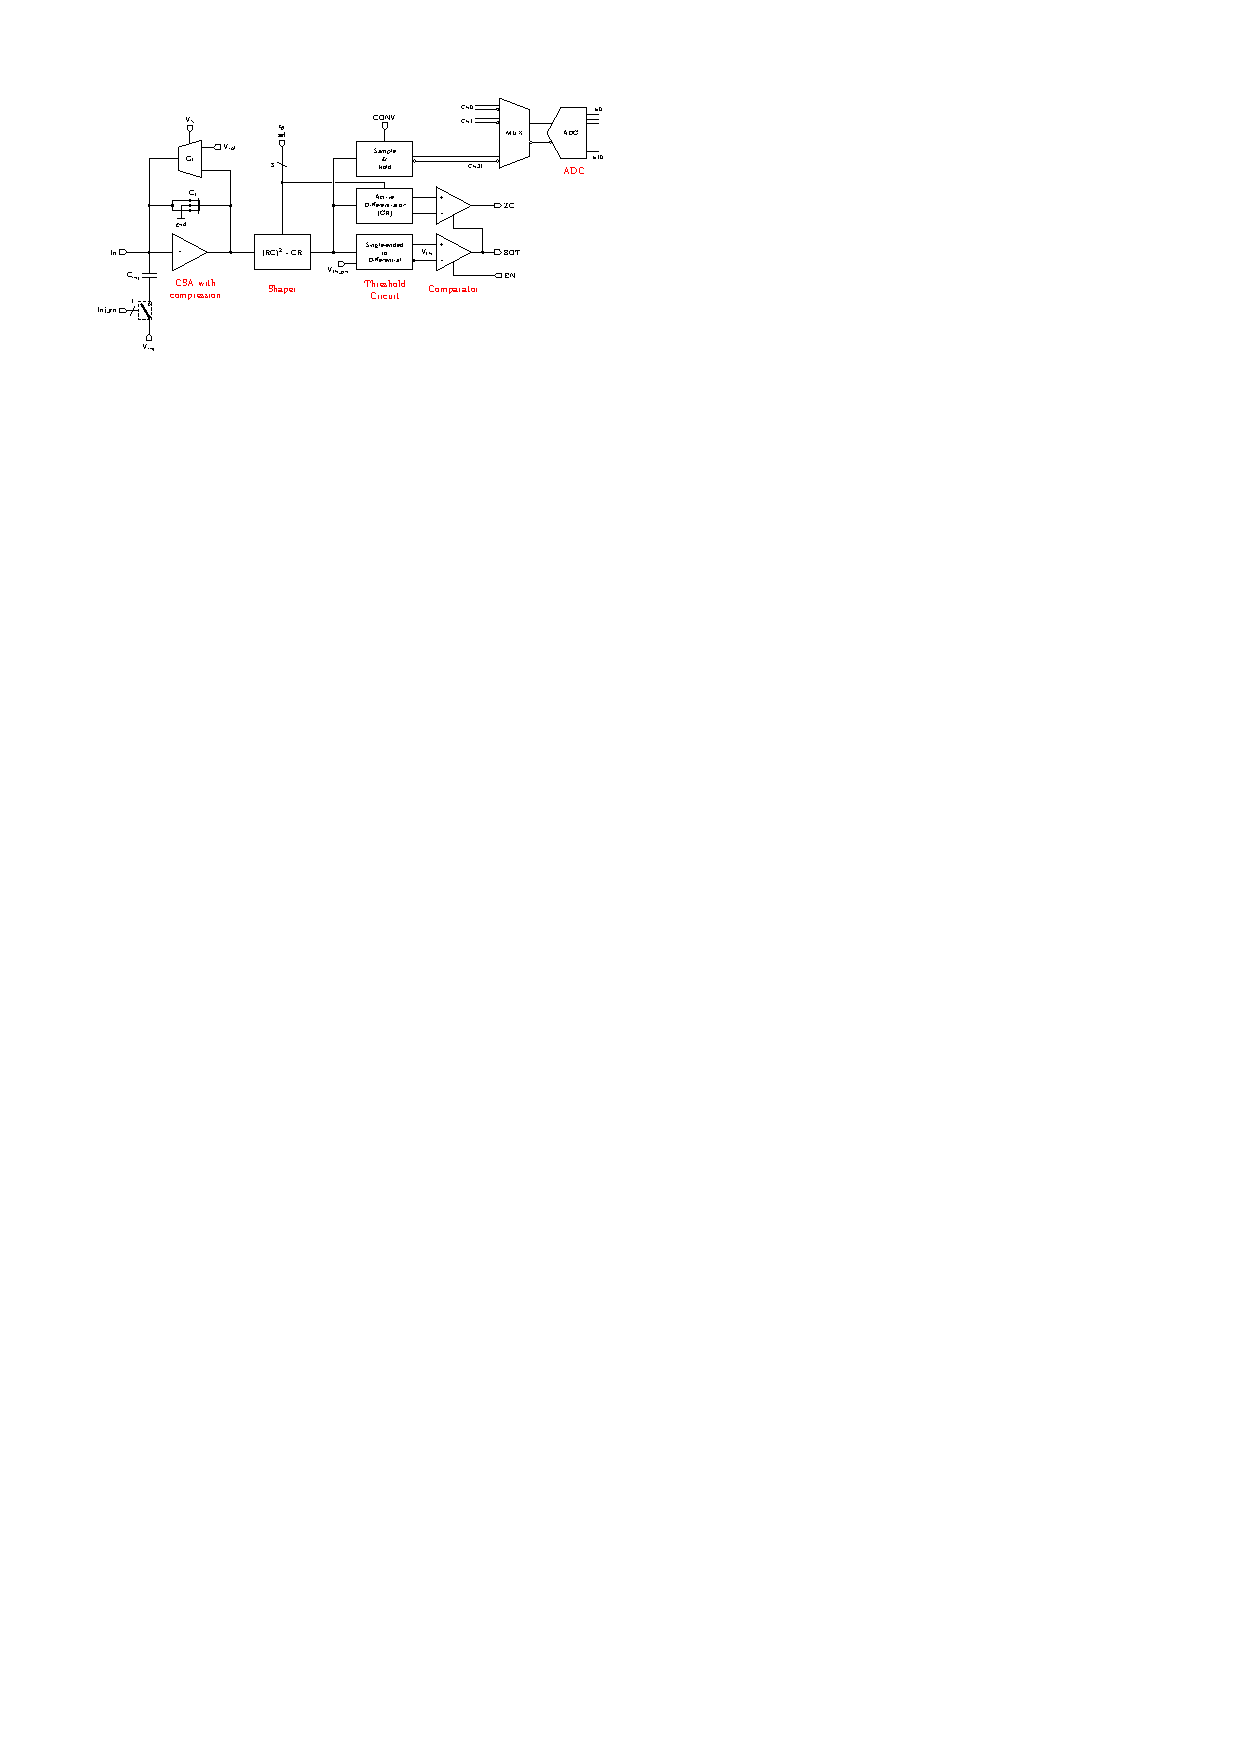
\includegraphics[width=0.68\textwidth]{images/backup_slides/readoutchannelADC.pdf}

    \vskip0.2cm
    
    \begin{columns}[T]
        \column{0.3\textwidth}
            \begin{itemize}
                \item \textbf{Charge Sensitive Amplifier}\\ with dynamic signal compression
                \item \textbf{CR-(RC)$^{2}$ filter}\\ with 8 selectable peaking times (from \SI{250}{\nano\second} to \SI{1.8}{\micro\second})
            \end{itemize}
            
        \column{0.36\textwidth}
            \begin{itemize}
                \item \textbf{SOT comparator}\\ Signal Over Threshold identification
                \item \textbf{Active CR and ZC comparator}\\ Shaper signal peak detection
                \item \textbf{Single-ended to differential S\&H}\\ Shaper signal peak storage
            \end{itemize}
        
        \column{0.25\textwidth}
            \begin{itemize}
                \item \textbf{Injection capacitance $C_{inj}$}\\ Used for calibration
                \item \textbf{11-bit hybrid SAR ADC} \\ One per ASIC with 32:1 multiplexer
            \end{itemize}
    \end{columns}
\end{frame}
}

\backupend

\end{document}